\documentclass[11pt]{article}
\usepackage[margin=0.75in]{geometry}
\usepackage{amsmath}
\usepackage{enumitem}
\usepackage{color,soul}
\usepackage{multicol}
\usepackage{tikz}

\newcommand{\ds}{\displaystyle}

\begin{document}
\newcounter{enumCount}
\pagestyle{empty}
\subsection*{Math 141 - Homework 11 \hfill Name: \underline{\hspace*{2in}}}


\textit{Solve each of the following optimization problems.  Be sure to include confirmation that your solution is really the maximum or the minimum (use the first or second derivative test).}

\begin{enumerate}
\item Two poles are connected by a wire that is also
connected to the ground. The first pole is 20 ft tall and
the second pole is 10 ft tall. There is a distance of 30 ft
between the two poles. Where should the wire be anchored
to the ground to minimize the amount of wire needed?
\begin{flushright}
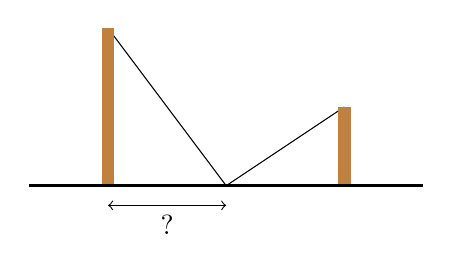
\begin{tikzpicture}
\draw (3,1) -- (1.5,0) -- (0,2);

\draw[<->] (0,-0.25) -- (0.75,-0.25) node[below] {?} -- (1.5,-0.25);
\fill[brown] (-0.08,0) rectangle (0.08,2);
\fill[brown] (2.92,0) rectangle (3.08,1);
\draw[very thick] (-1,0) -- (4,0);
\end{tikzpicture}
\end{flushright}
\vfill

\item The sum of two positive numbers is 10.  Find the values of the numbers that maximize their product.  
\vfill
\vfill

\item What point on the line $3x + 4y = 50$ is closest to the origin? 
\vfill
\vfill

\item A Norman window is a rectangle with a half-circle on top. If the perimeter of the window is 20 feet, find the dimensions $r$ and $h$ for the Norman window that has the largest possible area. 
\begin{flushright}
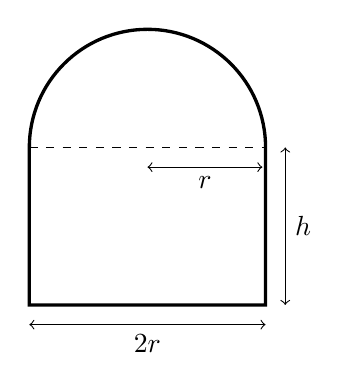
\begin{tikzpicture}
\draw[very thick] (0,0) -- (3,0) -- (3,2) arc (0:180:1.5) -- cycle;
\draw[dashed] (0,2) -- (3,2);
\draw[<->] (0,-0.25) -- (1.5,-0.25) node[below] {$2r$} -- (3,-0.25);
\draw[<->] (1.5,1.75) -- (2.23,1.75) node[below] {$r$} -- (2.96,1.75);
\draw[<->] (3.25,0) -- (3.25,1) node[right] {$h$} -- (3.25,2);
\end{tikzpicture}
\end{flushright}

\newpage
\item A farmer has 600 feet of fencing and wants to create a rectangular enclosure with a fence dividing the middle.  Find the dimensions of the enclosure that maximize the area.  
\begin{flushright}
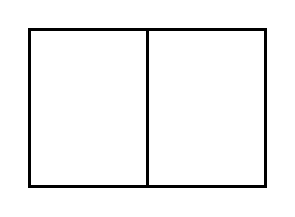
\begin{tikzpicture}
\draw[very thick] (0,0) rectangle (3,2);
\draw[very thick] (1.5,0) -- (1.5,2);
\end{tikzpicture}
\end{flushright}
\vfill

\item In economics, if $C(x)$ is the cost to produce $x$ units of a commodity, then $\dfrac{C(x)}{x}$ is the \textbf{average cost} per unit produced.  The derivative $C'(x)$ is the \textbf{marginal cost} of each extra item. Use calculus to show that the average cost is minimized at a level of production $x$ where the average cost is equal to the marginal cost.   
\vfill


\item The trapezoid shown below has 3 short sides that are all 10 cm long and one long base.  Find the angle $\theta$ that maximizes the area of the trapezoid.  Recall that the area of a trapezoid is $A = \tfrac{1}{2} (a + b) h$ where $a$ is the length of the top side, $b$ is the length of the base, and $h$ is the height (the distance from the top to the bottom). 
\begin{flushright}
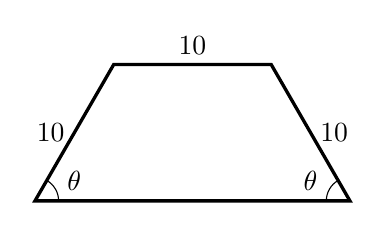
\begin{tikzpicture}[scale=0.2]
\draw (10,8.66) node[above] {10};
\draw (2.5,4.33) node[left] {10};
\draw (17.5,4.33) node[right] {10};
\draw[very thick] (0,0) -- (5,8.66) -- (15,8.66) -- (20,0) -- cycle;
\draw (0,0) node[xshift=0.5cm, yshift=0.25cm] {$\theta$};
\draw (20,0) node[xshift=-0.5cm, yshift=0.25cm] {$\theta$};
\draw (0:1.5) arc(0:60:1.5);
\draw (18.5,0) arc(180:120:1.5);
\end{tikzpicture}
\end{flushright}
\vfill

\item A rectangle is inscribed in a quarter circle of radius 2 (shown below).  Use calculus to show that the area of the rectangle is maximized when $\theta = \tfrac{\pi}{4}$.
\begin{flushright}
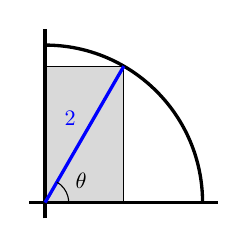
\begin{tikzpicture}[scale=1.0]
\filldraw[fill=gray!30] (0,0) rectangle (1,1.732);
\draw[very thick] (-0.2,0) -- (2.2,0);
\draw[very thick] (0,-0.2) -- (0,2.2);
\draw[very thick] (2,0) arc(0:90:2);
\draw[very thick, blue] (0,0) -- (0.5, 0.866) node[above left,scale=0.8] {2} -- (1,1.732);
\draw (0.3,0) arc (0:15:0.3) node[above right,scale=0.8] {$\theta$} arc(15:60:0.3);
\end{tikzpicture}
\end{flushright}
\vfill

\end{enumerate}

\end{document}
